\documentclass[11pt,letterpaper]{article}

\usepackage{graphicx}
\usepackage[margin=1in]{geometry}
\usepackage{amsmath}
\usepackage[T1]{fontenc}
\usepackage[utf8]{inputenc}
\usepackage{authblk}
\usepackage{fancyhdr}
\usepackage{lastpage}
\usepackage[parfill]{parskip}
\usepackage{subcaption}

\pagestyle{fancyplain}

% Headers
\lhead{}
\chead{}
\rhead{}

% Footers
\lfoot{}
\cfoot{}
\rfoot{\footnotesize Page \thepage\ of \pageref{LastPage}}

\renewcommand{\headrulewidth}{0.0pt} % No header rule
\renewcommand{\footrulewidth}{0.4pt} % Thin footer rule

\title{Consistency Simulations: Raft vs. Eventual}
\date{August 25, 2016}
\author[ ]{Benjamin Bengfort}
\author[ ]{Pete Keleher}
\affil[ ]{Department of Computer Science}
\affil[ ]{University of Maryland}
\affil[ ]{\textit{\{bengfort,keleher\}@cs.umd.edu}}

\begin{document}

\maketitle

In these results we present the performance of homogenous Raft and Eventual systems with an increasing number of nodes. In particular the goal of this report is to observe the relative performance of each type of system as the system is scaled with respect to several metrics.

The simulation settings were fairly conservative in order to promote a quick simulation result, particularly with respect to latency. Most simulation settings are specified in Table \ref{table:settings}.

\begin{table}[!h]
\makebox[\textwidth][c]{
\centering
\begin{tabular}{|r|ll|}
\hline
setting              & raft                      & eventual                  \\
\hline
Nodes                & 5, 25, 50, 75, 100        & 5, 25, 50, 75, 100        \\
Links                & 20, 600, 2450, 9900, 5550 & 20, 600, 2450, 9900, 5550 \\
Local Latency ($\mu$, $\sigma$) & (100, 5)       & (100, 5)                  \\
Wide Latency ($\mu$, $\sigma$) & (1000, 56)      & (1000, 56)                \\
Latency Range        & 888-1112ms                & 888-1112ms                \\
Tick Metric $T$      & 10000                     & 10000                     \\
Tick Model           & bailis                    & bailis                    \\
Election Timeout     & U(10000, 20000)           & N/A                       \\
Heartbeat Interval   & 5000ms                    & N/A                       \\
Anti-Entropy Delay   & N/A                       & 2500ms                    \\
AE Neighbors ($n$)   & N/A                       & 1                         \\
$P_{sync}$           & N/A                       & N/A                       \\
$P_{local}$          & N/A                       & 0.6                       \\
$P_{conflict}$       & 0.5                       & 0.5                       \\
$P_{read}$           & 0.58                      & 0.58                      \\
Access Interval ($\mu$, $\sigma$) & (1800, 240)  & (1800, 240)               \\
Objects              & 55, 69, 77, 75, 100       & 55, 69, 77, 75, 100       \\
Access per Object    & 80                        & 80                        \\
Writes               & 12,014 - 240,047          & 12,014 - 240,047          \\
\hline
\end{tabular}}
\caption{\textsf{Static settings aggregated by Replica/Experiment type.}}
\label{table:settings}
\end{table}

\begin{figure}[!h]
    \centering
        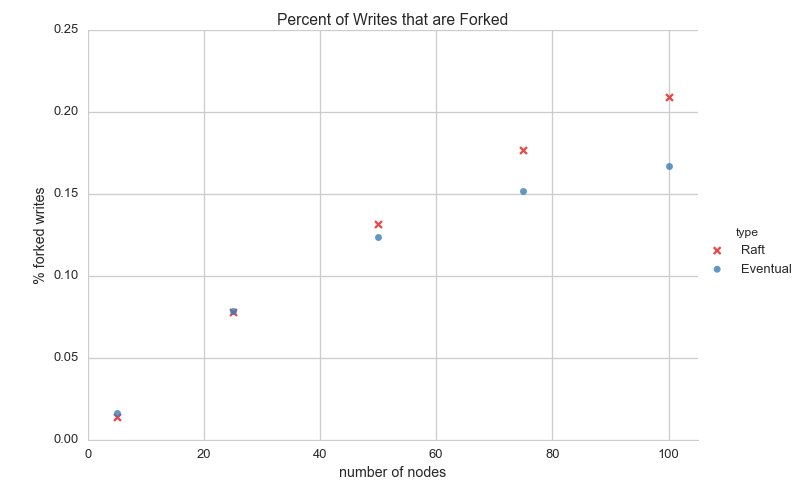
\includegraphics[width=\textwidth]{figures/forked_writes.png}
        \caption{\textsf{As the system grows there is a higher likelihood of forks because there are more nodes writing to about the same number of objects. Beyond this static increase in likelihood, we were also expecting that Eventual would have more forks than Raft at the higher number of nodes because of the longer convergence time, e.g. the longer the convergence time the likelihood of a fork also increases. However, this shows that the more nodes there are, Raft has more forks, implying that Eventual converges more quickly than the broadcast AppendEntries even at 100 nodes.}}
        \label{fig:forked_writes}
\end{figure}

\begin{figure}[!h]
    \centering
        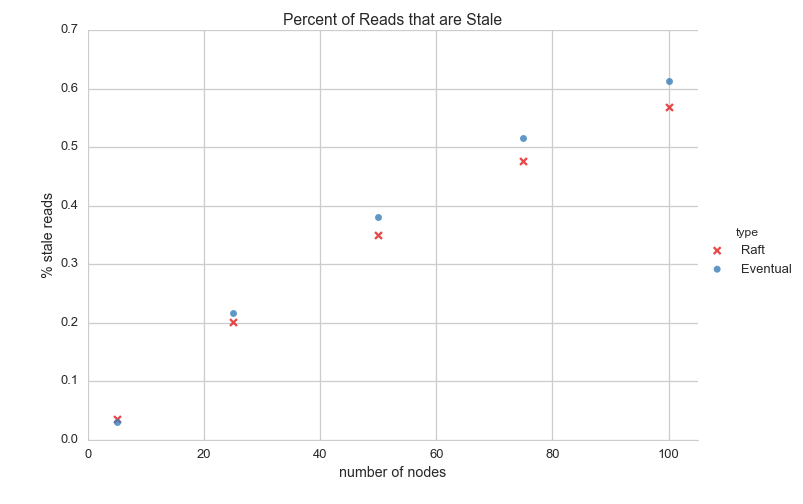
\includegraphics[width=\textwidth]{figures/stale_reads.png}
        \caption{\textsf{As the system grows, there is a higher likelihood that a newer version exists somewhere in the system that hasn't propagated, and as you can see after about 70 nodes in our system, the majority of reads are stale. These numbers should parallel the forked writes (a forked write is a write that follows a stale read), however here Eventual is doing worse than Raft, though they are fairly close together. Perhaps we need to increase the amount of conflict in order to get a better feel for what is happening.}}
        \label{fig:stale_reads}
\end{figure}

\begin{figure}[!h]
    \centering
        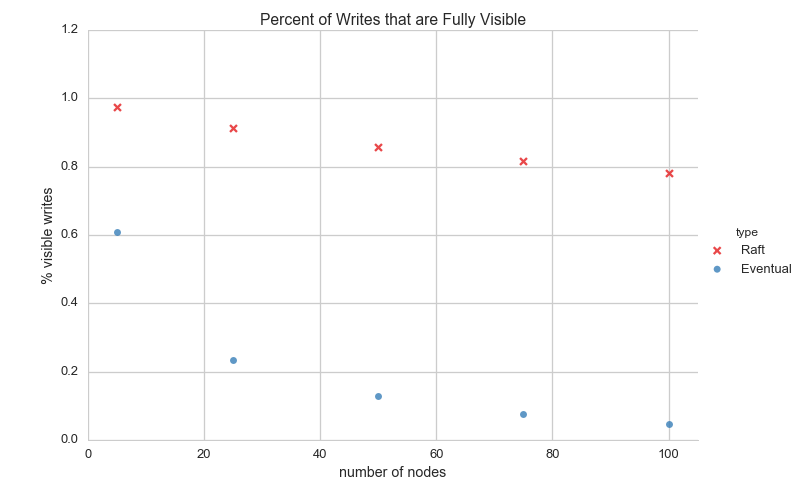
\includegraphics[width=\textwidth]{figures/visible_writes.png}
        \caption{\textsf{Raft achieves close to 100\% visibility as it uses broadcast from the leader to push all writes to all nodes (only dropped writes are not made fully visible). Even with 5 nodes, Eventual cannot get full visibility as later writes stomp on the replication of older writes. This effect increases dramatically the more nodes there are.}}
        \label{fig:visible_writes}
\end{figure}

\begin{figure}[!h]
    \centering
        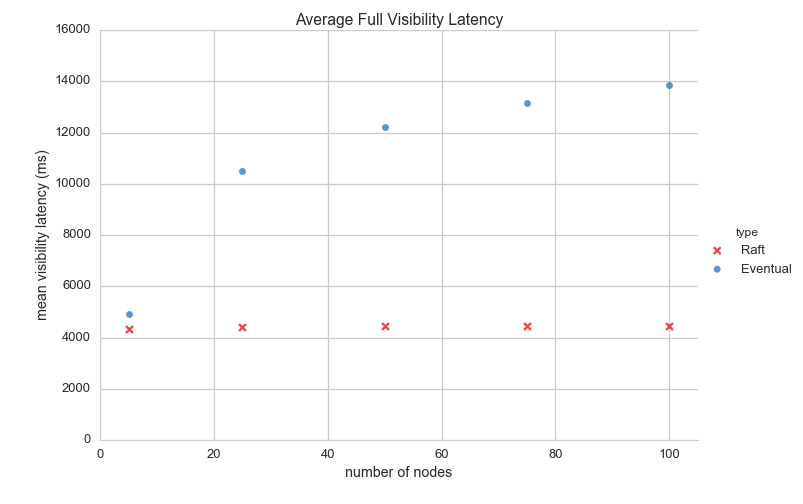
\includegraphics[width=\textwidth]{figures/visibility_latency.png}
        \caption{\textsf{Because Raft is broadcast, writes become visible within a heartbeat interval (a bit less for writes that originate at the leader). The latency continues to increase for Eventual the more nodes there are as the system is working to converge across the entire network.}}
        \label{fig:visibility_latency}
\end{figure}

\begin{figure}[!h]
    \centering
        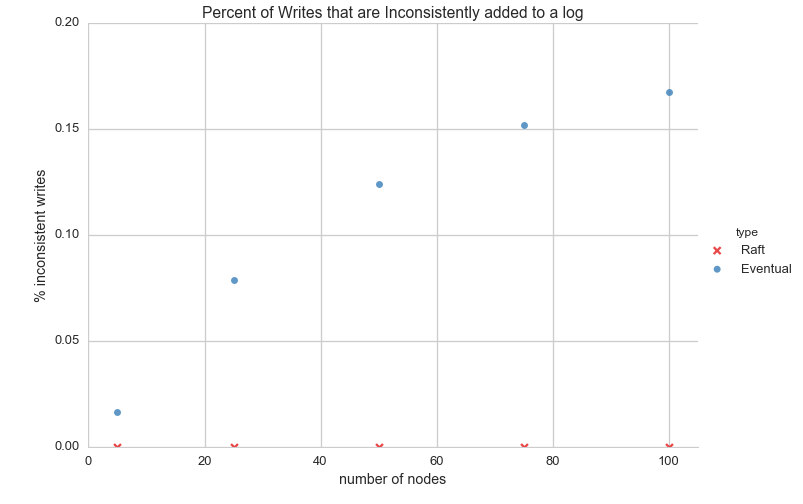
\includegraphics[width=\textwidth]{figures/inconsistent_writes.png}
        \caption{\textsf{Raft will not allow an inconsistent write by dropping it, however every Eventual fork is an inconsistent write.}}
        \label{fig:inconsistent_writes}
\end{figure}

\begin{figure}[!h]
    \centering
        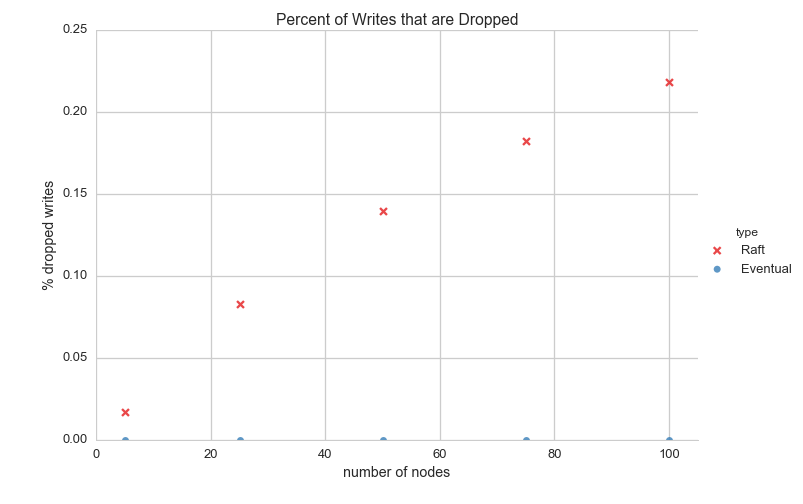
\includegraphics[width=\textwidth]{figures/dropped_writes.png}
        \caption{\textsf{Raft should drop 100\% of its forks, Eventual drops none.}}
        \label{fig:dropped_writes}
\end{figure}

\begin{figure}[!h]
    \centering
        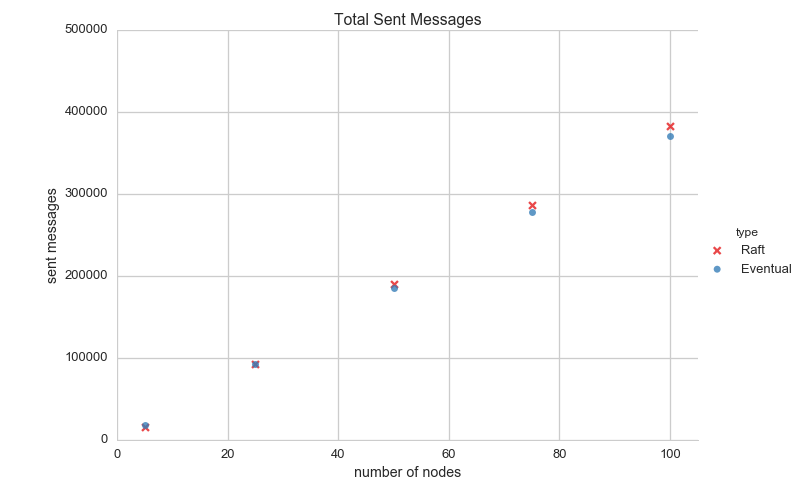
\includegraphics[width=\textwidth]{figures/messages_sent.png}
        \caption{\textsf{In these simulations both Raft and Eventual have a fixed communication budget that is defined by the relationship of their timing parameters (anti-entropy delay and heartbeat interval).}}
        \label{fig:messages_sent}
\end{figure}

\begin{figure}[!h]
    \centering
        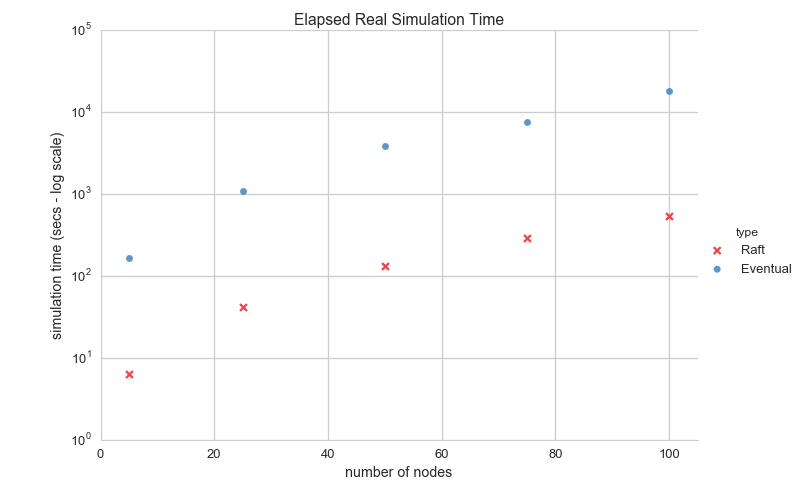
\includegraphics[width=\textwidth]{figures/simulation_time.png}
        \caption{\textsf{The more nodes, the longer the simulation (note the logarithmic scale) -- Eventual appears to be a fixed amount of time longer than Raft.}}
        \label{fig:simulation_time}
\end{figure}

\begin{figure}[!h]
    \centering
        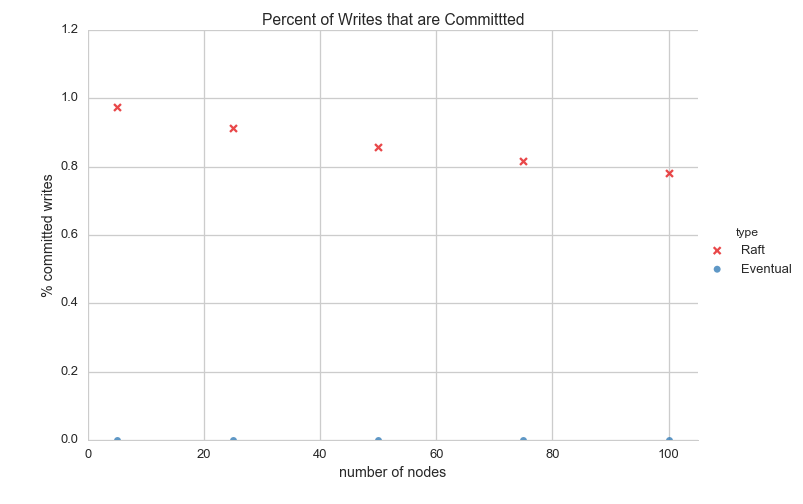
\includegraphics[width=\textwidth]{figures/committed_writes.png}
        \caption{\textsf{Raft commits nearly all writes (except those that it drops). Eventual commits none.}}
        \label{fig:committed_writes}
\end{figure}

\begin{figure}[!h]
    \centering
        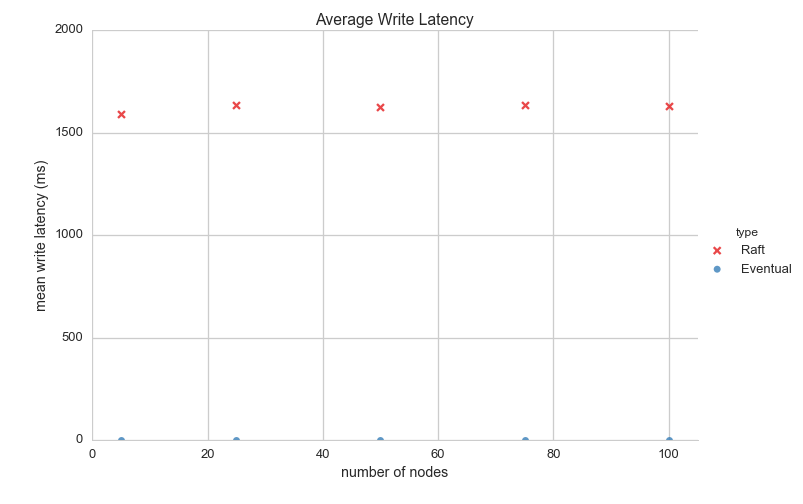
\includegraphics[width=\textwidth]{figures/write_latency.png}
        \caption{\textsf{The write latency embeds the amount of time for a \texttt{RemoteWrite} to the leader and the response. Eventual writes locally, immediately therefore there is no write latency.}}
        \label{fig:write_latency}
\end{figure}

\begin{figure}[!h]
    \centering
        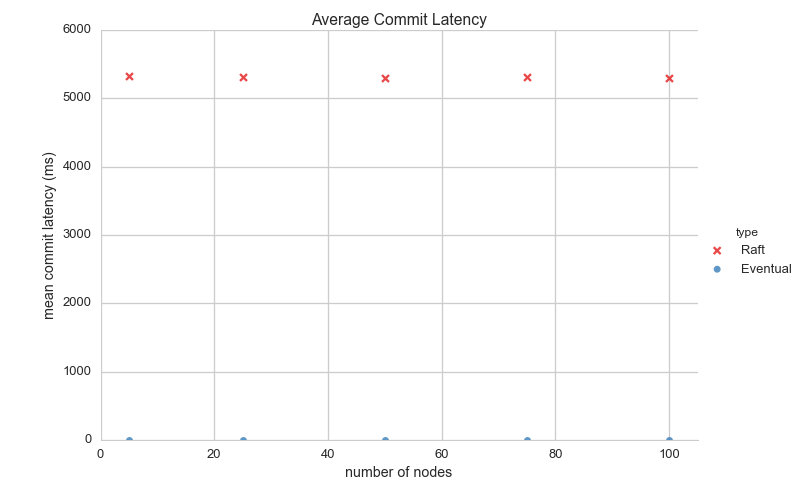
\includegraphics[width=\textwidth]{figures/commit_latency.png}
        \caption{\textsf{The commit latency is approximately the remote write latency plus a heartbeat interval, given no outages.}}
        \label{fig:commit_latency}
\end{figure}

\begin{figure}[!h]
    \centering
        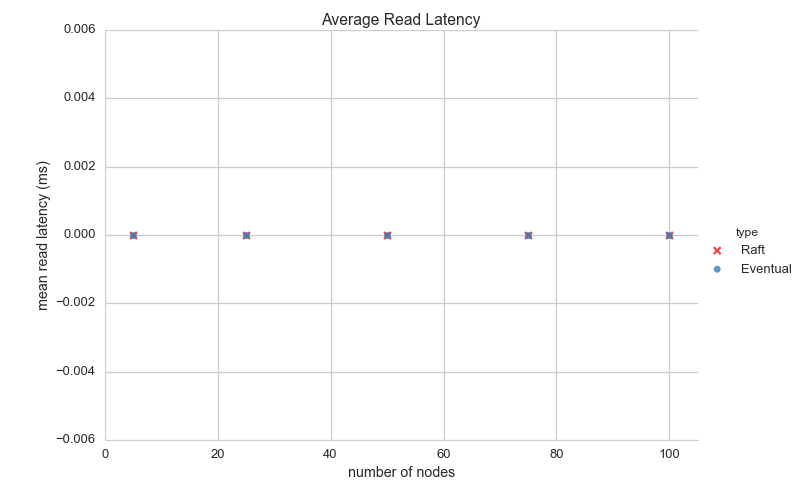
\includegraphics[width=\textwidth]{figures/read_latency.png}
        \caption{\textsf{Every node implements read local cache, therefore every node has zero read latency.}}
        \label{fig:read_latency}
\end{figure}

\begin{figure}[!h]
    \centering
        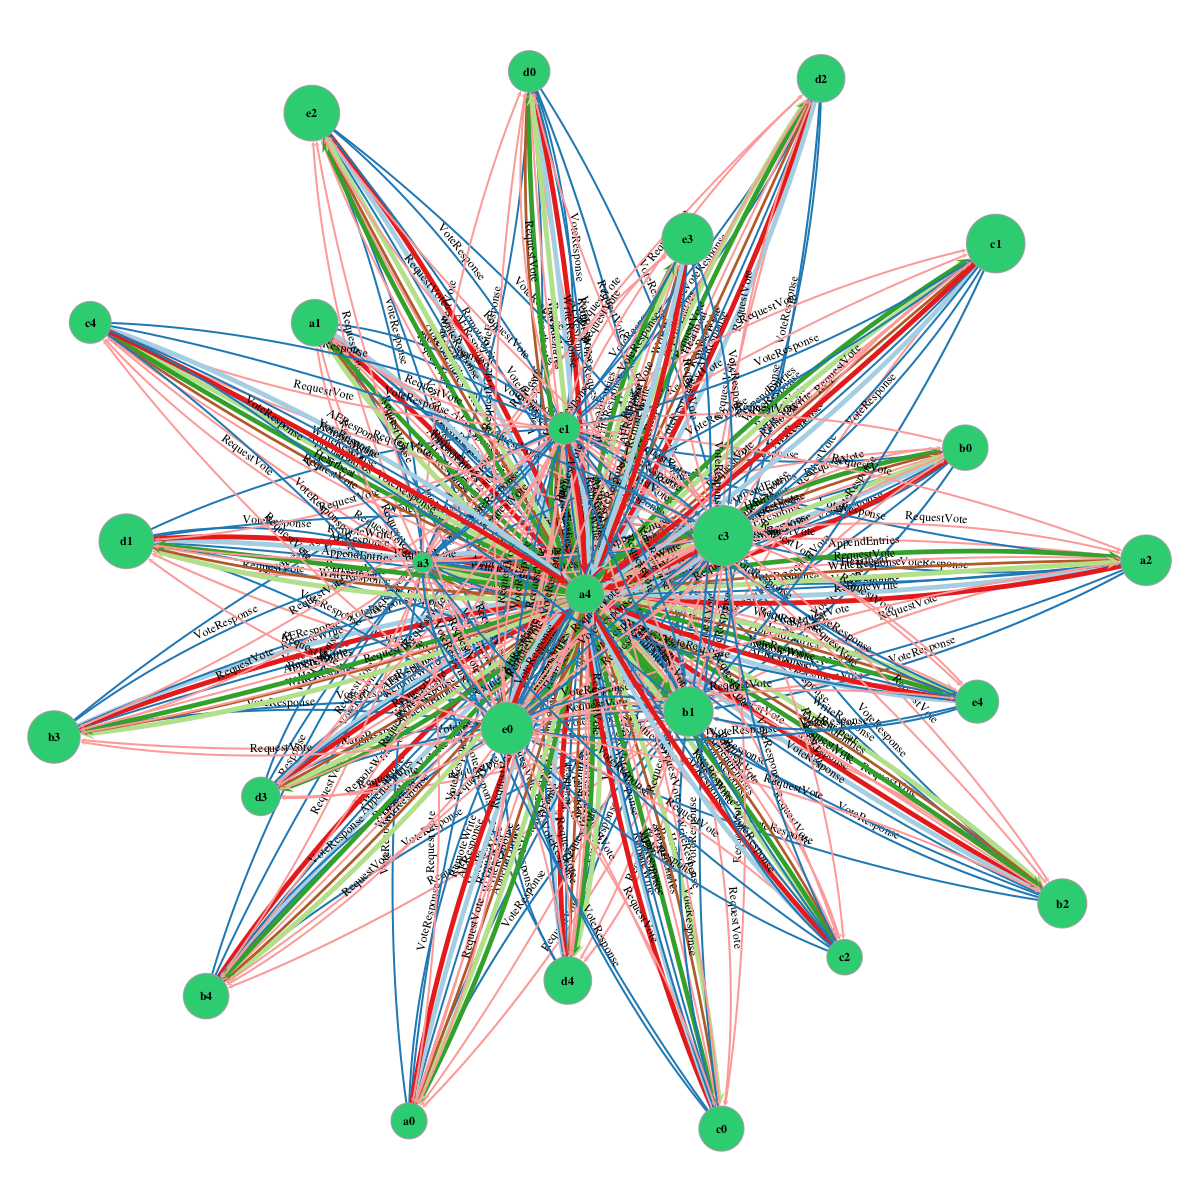
\includegraphics[width=\textwidth]{figures/raft-25users.png}
        \caption{\textsf{A graph of messages in the 25 Raft system. The size of the vertex is the number of writes, the edges are colored and labeled by message type and the size of the edge relates to the number of messages sent. Nodes are positioned based on how many messages they send. It is clear which node is the leader in this figure.}}
        \label{fig:topology}
\end{figure}

\begin{figure}[!h]
    \centering
        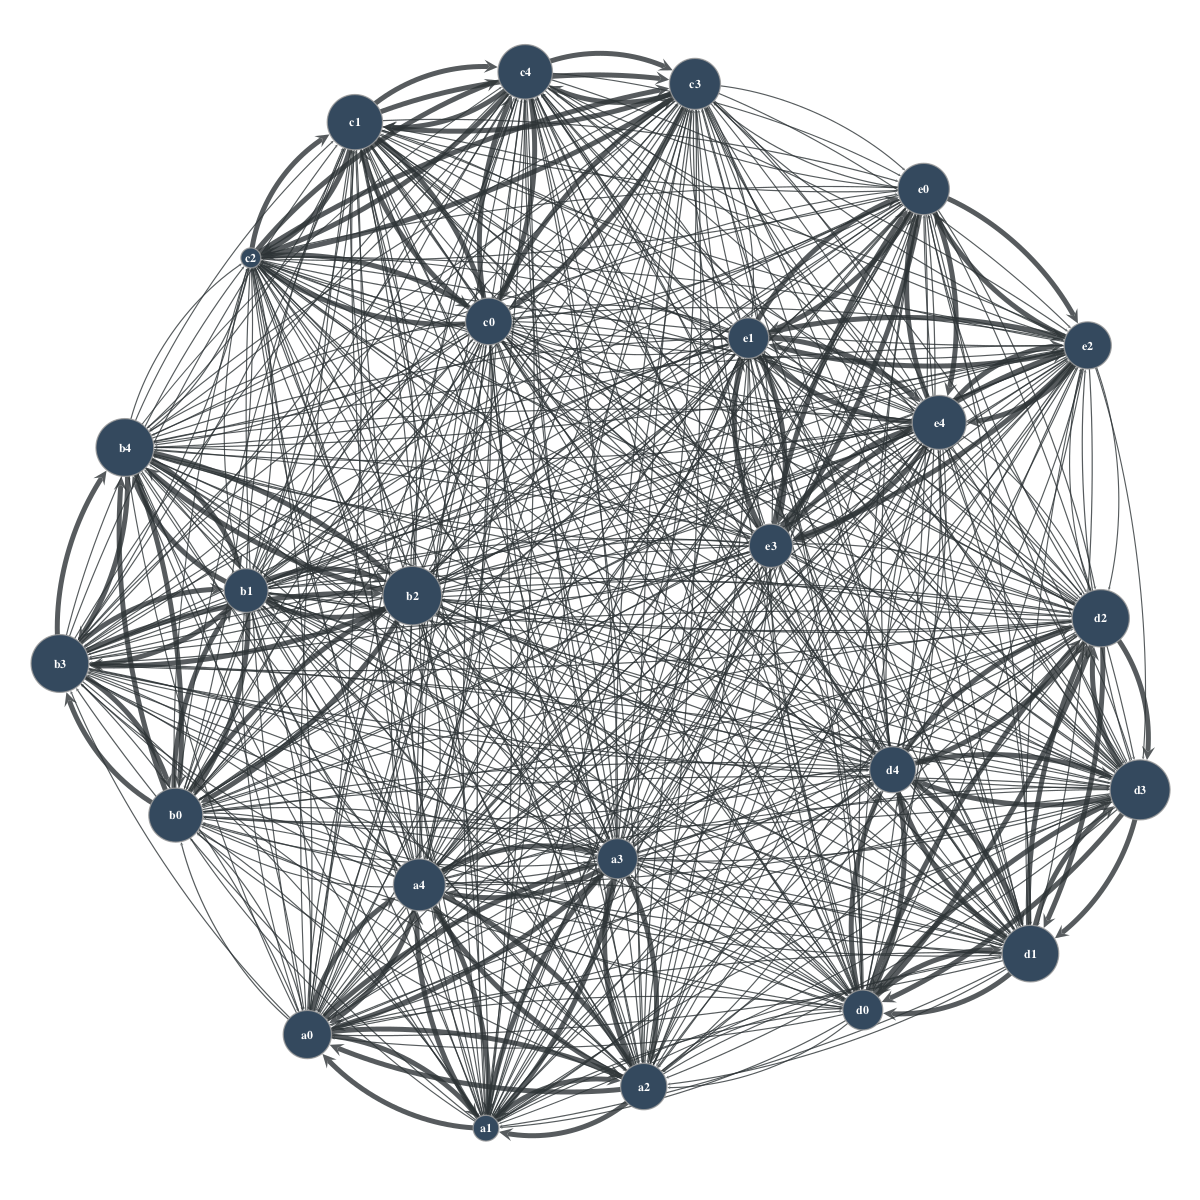
\includegraphics[width=\textwidth]{figures/eventual-25nodes.png}
        \caption{\textsf{This is the measured latency graph. The size of the node relates to the number of messages sent. The edge size is the mean latency, where thicker edges mean a lower mean latency (measured) and nodes are positioned according to latency as well.}}
        \label{fig:topology}
\end{figure}

\begin{figure}[!h]
    \centering
        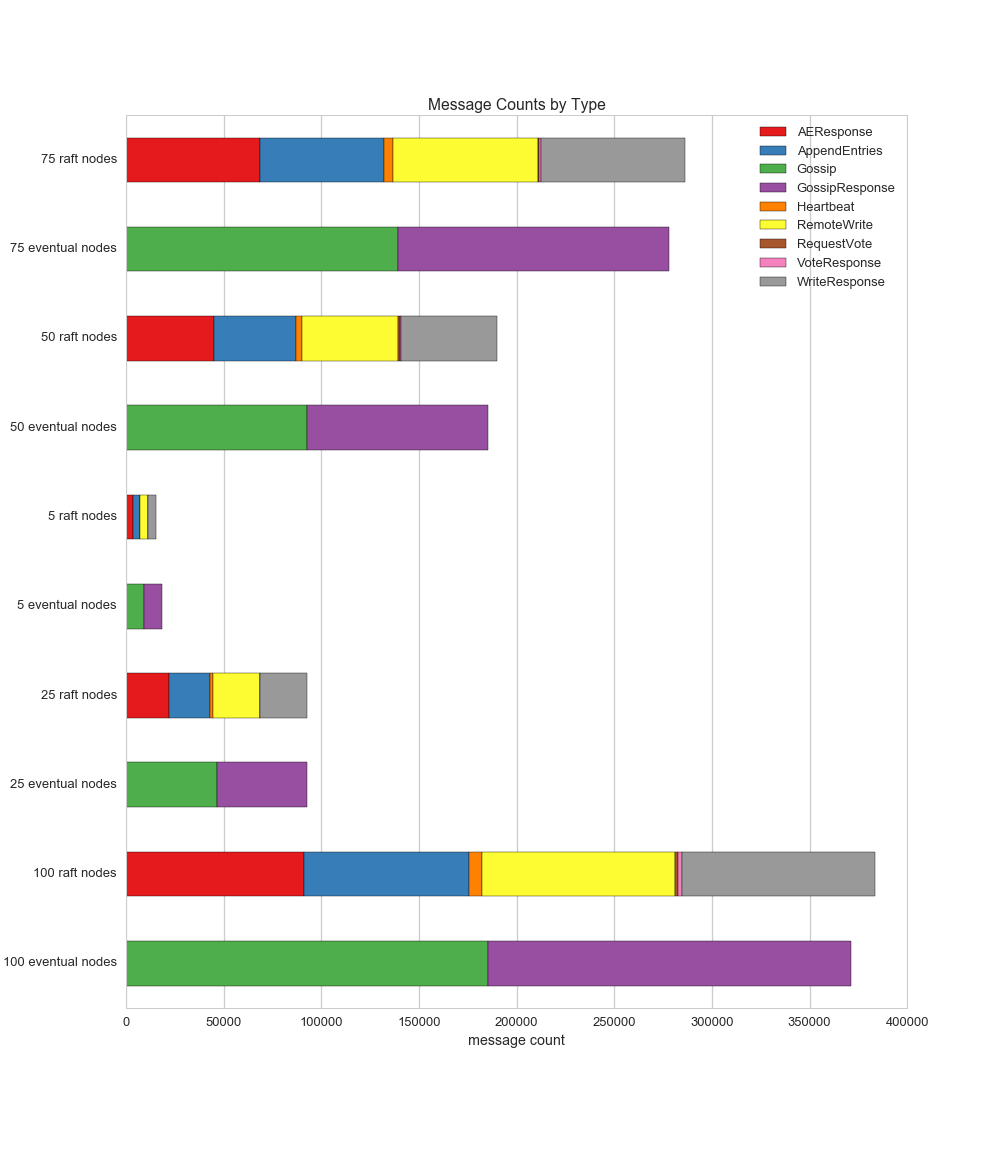
\includegraphics[height=.9\textheight]{figures/message_counts.png}
        \caption{\textsf{See \ref{fig:messages_sent} for more details.}}
        \label{fig:message_counts}
\end{figure}

\end{document}
